\documentclass[a4paper,12pt]{article}
\usepackage[brazil]{babel}
\usepackage[utf8]{inputenc}
\usepackage[T1]{fontenc}
\usepackage{geometry}
\usepackage{setspace}
\usepackage{titlesec}
\usepackage{hyperref}
\usepackage{graphicx}
\usepackage{caption}
\usepackage{subcaption}
\usepackage{fancyhdr}
\usepackage{xcolor}

%%%%%%%%%%%%%%%%%%%%%%%%%%%%%%%%%%%%%%%%%%%%%%%%%%
% These are some new commands that may be useful 
% for paper writing in general. If other new commands
% are needed for your specific paper, please feel 
% free to add here. 
%
% The currently available commands are organized in: 
% 1) Systems
% 2) Quantities
% 3) Energies and units
% 4) particle species
% 5) Colors package
% 6) hyperlink
%%%%%%%%%%%%%%%%%%%%%%%%%%%%%%%%%%%%%%%%%%%%%%%%%%

\usepackage{amsmath}
\usepackage{amssymb}
\usepackage{upgreek}
\usepackage{multirow}
\usepackage{setspace}% http://ctan.org/pkg/setspace
\usepackage{fancyhdr}
\usepackage{datetime}

% 1) SYSTEMS
\newcommand{\btc}               {\textbf{BTC}}
\newcommand{\btcspace}          {\textbf{BTC} }
\newcommand{\pow}               {\textbf{PoW}}

% 4) definition to references, biblatex and hyperlink
\usepackage[backend=bibtex, 
style=nature,  %style reference.
sorting=none,
firstinits=true %first name abbreviate
]{biblatex}

\usepackage{hyperref}
\hypersetup{
    colorlinks=true, %set "true" if you want colored links
    linktoc=all,     %set to "all" if you want both sections and subsections linked
    linkcolor=blue,  %choose some color if you want links to stand out
    citecolor= blue, % color of \cite{} in the text.
    urlcolor  = blue, % color of the link for the paper in references.
}

% 5) Tikz and figures
\usepackage{epsfig}
\usepackage{lmodern}
\usepackage{mathtools}
\usepackage[utf8]{luainputenc}
\usepackage{xspace}
\usepackage{tikz}
\usepackage{pgfplots}
\pgfplotsset{compat=newest}

\usetikzlibrary{positioning}
\usepackage{subcaption}

% 6) colors:
\usepackage{xcolor}
\definecolor{ao(english)}{rgb}{0.0, 0.5, 0.0} % dark green

% 7) Add lines numbers
%\usepackage{lineno}

% add pdf file to thesis:
\usepackage{pdfpages}

\usepackage[most]{tcolorbox}

%textmarker style from colorbox doc
\tcbset{textmarker/.style={%
        enhanced,
        parbox=false,boxrule=0mm,boxsep=0mm,arc=0mm,
        outer arc=0mm,left=6mm,right=3mm,top=7pt,bottom=7pt,
        toptitle=1mm,bottomtitle=1mm,oversize}}


% define new colorboxes
\newtcolorbox{hintBox}{textmarker,
    borderline west={6pt}{0pt}{yellow},
    colback=yellow!10!white}
\newtcolorbox{importantBox}{textmarker,
    borderline west={6pt}{0pt}{red},
    colback=red!10!white}
\newtcolorbox{noteBox}{textmarker,
    borderline west={6pt}{0pt}{green},
    colback=green!10!white}

% define commands for easy access
\newcommand{\note}[1]{\begin{noteBox} \textbf{} #1 \end{noteBox}}
\newcommand{\warning}[1]{\begin{hintBox} \textbf{Warning:} #1 \end{hintBox}}
\newcommand{\important}[1]{\begin{importantBox} \textbf{} #1 \end{importantBox}}

\hypersetup{
    colorlinks=true,% make the links colored
    linkcolor=blue
}

\usepackage{setspace}
\addbibresource{bibliography.bib}

\newcommand{\printingbibliography}{%

    \pagestyle{myheadings}
    \markright{}
    \sloppy
    \printbibliography[heading=bibintoc, % add to table of contents
                   title=Refer\^encias % Chapter name
                  ]
    \fussy%
}
\PassOptionsToPackage{table}{xcolor}
\renewcommand{\baselinestretch}{1.5}

\pagestyle{fancy}
\fancyhf{}
\renewcommand{\headrulewidth}{0pt}
\fancyhead[R]{\thepage}

\geometry{a4paper,top=30mm,bottom=20mm,left=30mm,right=20mm}

\titleformat*{\section}{\bfseries\large}
\titleformat*{\subsection}{\bfseries\normalsize}

\title{}
\author{Andr\'e V. Silva}
\date{\today}

\begin{document}

\maketitle

\begin{figure}[!h]
\centering
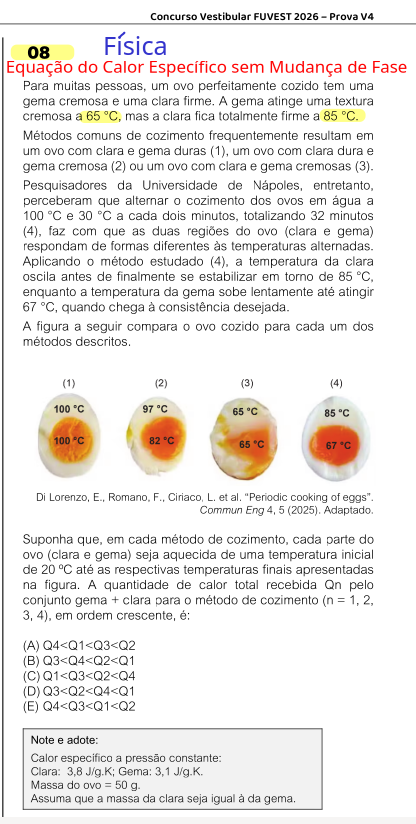
\includegraphics[width=0.7\textwidth]{images/8.png}
\caption{Figura 1}
\end{figure}

\newpage

\subsection*{Resolução}

A quantidade de calor recebida é dada por:
\[
Q = m \, c \, \Delta T
\]

Como a massa da clara é igual à da gema:
\[
m_{\text{clara}} = m_{\text{gema}} = \frac{50}{2} = 25\,g
\]

Dados:
\[
c_{\text{clara}} = 3{,}8 \, \text{J/g.K}, \quad
c_{\text{gema}} = 3{,}1 \, \text{J/g.K}
\]

Temperatura inicial:
\[
T_i = 20^\circ C
\]

Agora calculamos $Q$ para cada método:

\paragraph{Método (1)}
\[
T_{\text{clara}} = 100^\circ C, \quad T_{\text{gema}} = 100^\circ C
\]

\[
Q_1 = 25 \cdot 3{,}8 \cdot (100-20) + 25 \cdot 3{,}1 \cdot (100-20)
\]

\[
Q_1 = 25 \cdot 3{,}8 \cdot 80 + 25 \cdot 3{,}1 \cdot 80
\]

\[
Q_1 = 7600 + 6200 = 13800 \, \text{J}
\]

\paragraph{Método (2)}
\[
T_{\text{clara}} = 97^\circ C, \quad T_{\text{gema}} = 82^\circ C
\]

\[
Q_2 = 25 \cdot 3{,}8 \cdot (97-20) + 25 \cdot 3{,}1 \cdot (82-20)
\]

\[
Q_2 = 25 \cdot 3{,}8 \cdot 77 + 25 \cdot 3{,}1 \cdot 62
\]

\[
Q_2 = 7315 + 4805 = 12120 \, \text{J}
\]

\paragraph{Método (3)}
\[
T_{\text{clara}} = 65^\circ C, \quad T_{\text{gema}} = 65^\circ C
\]

\[
Q_3 = 25 \cdot 3{,}8 \cdot (65-20) + 25 \cdot 3{,}1 \cdot (65-20)
\]

\[
Q_3 = 25 \cdot 3{,}8 \cdot 45 + 25 \cdot 3{,}1 \cdot 45
\]

\[
Q_3 = 4275 + 3487{,}5 = 7762{,}5 \, \text{J}
\]

\paragraph{Método (4)}
\[
T_{\text{clara}} = 85^\circ C, \quad T_{\text{gema}} = 67^\circ C
\]

\[
Q_4 = 25 \cdot 3{,}8 \cdot (85-20) + 25 \cdot 3{,}1 \cdot (67-20)
\]

\[
Q_4 = 25 \cdot 3{,}8 \cdot 65 + 25 \cdot 3{,}1 \cdot 47
\]

\[
Q_4 = 6175 + 3642{,}5 = 9817{,}5 \, \text{J}
\]

\paragraph{Ordem crescente de calor recebido:}
\[
Q_3 < Q_4 < Q_2 < Q_1
\]

\[
\boxed{(3) < (4) < (2) < (1)}
\]


\begin{figure}[!ht]
\centering
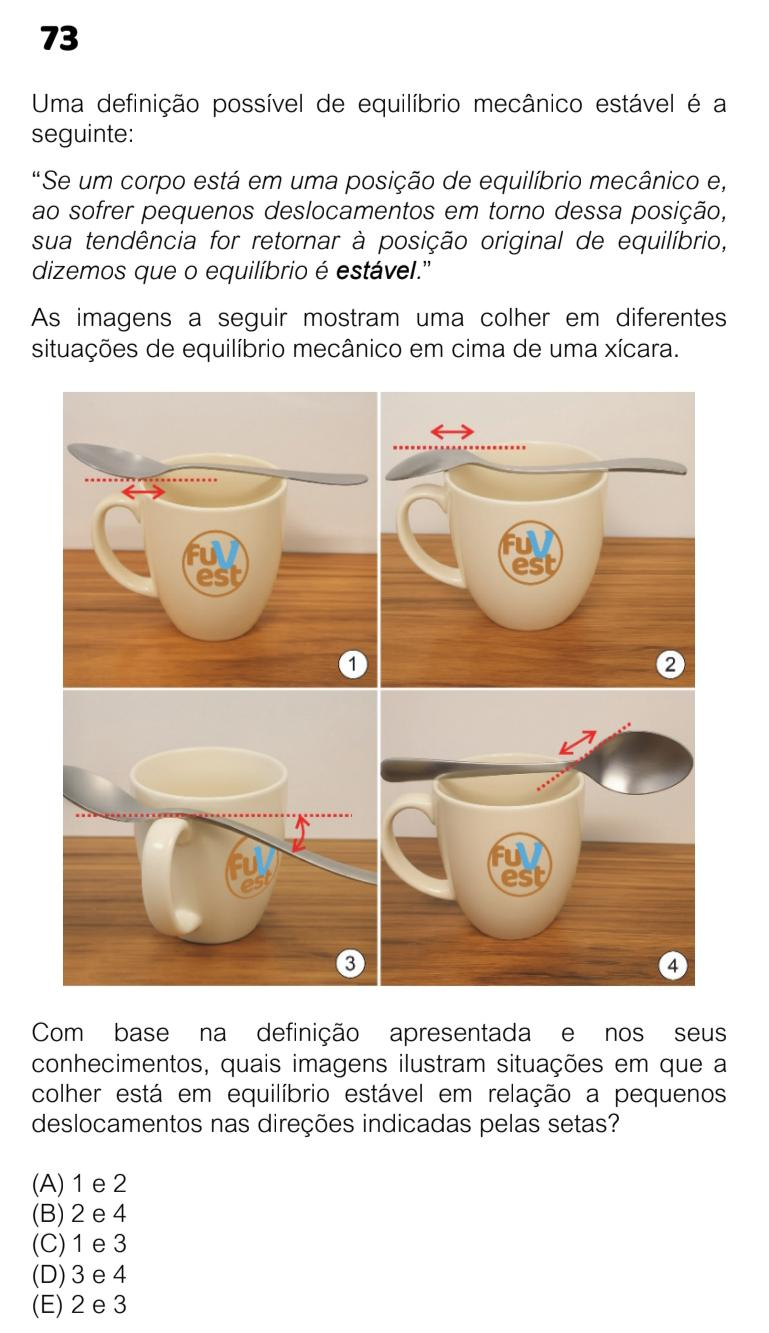
\includegraphics[width=0.65\textwidth]{images/1.png}
\caption{Colher em diferentes situações de equilíbrio sobre a xícara.}
\end{figure}


\begin{flushleft}

\textbf{\textcolor{blue}{\Large Quest\~ao 73}}\\

\vspace{0.3cm}

\textbf{Resolu\c{c}\~ao:}

\vspace{0.3cm}

O enunciado define \textbf{equilíbrio mecânico estável} como a situação em que, ao sofrer pequenos deslocamentos, o corpo tende a retornar à posição original.

\vspace{0.3cm}

Uma forma eficiente de analisar esse tipo de problema é por meio do \textbf{centro de massa (CM)} e da energia potencial gravitacional.

\begin{itemize}
\item Se, ao deslocar o corpo, o centro de massa \textbf{sobe}, o sistema retorna à posição inicial $\rightarrow$ equilíbrio estável.
\item Se o centro de massa \textbf{desce}, o sistema se afasta da posição inicial $\rightarrow$ equilíbrio instável.
\item Se a altura do centro de massa não se altera $\rightarrow$ equilíbrio indiferente.
\end{itemize}

\vspace{0.3cm}

\textbf{Análise das situações:}

\vspace{0.2cm}

\textbf{(1)} A colher está apoiada de forma que pequenos deslocamentos fazem o centro de massa descer, provocando queda.

\[
\Rightarrow \text{Equilíbrio instável}
\]

\vspace{0.2cm}

\textbf{(2)} A colher está bem posicionada sobre a borda da xícara. Pequenos deslocamentos fazem o centro de massa subir, gerando tendência de retorno.

\[
\Rightarrow \text{Equilíbrio estável}
\]

\vspace{0.2cm}

\textbf{(3)} A colher está em uma posição em que qualquer pequeno deslocamento faz o centro de massa descer, causando rotação e queda.

\[
\Rightarrow \text{Equilíbrio estável}
\]

\vspace{0.2cm}

\textbf{(4)} A colher está parcialmente apoiada dentro da xícara. Pequenos deslocamentos elevam o centro de massa, fazendo o sistema retornar à posição inicial.

\[
\Rightarrow \text{Equilíbrio instável}
\]

\vspace{0.5cm}

\textcolor{red}{\textbf{Conclus\~ao:}}\\

As situações em que a colher está em equilíbrio mecânico estável são:

\[
\boxed{2 \text{ e } 3}
\]

\vspace{0.3cm}

Portanto, a alternativa correta é \textbf{(B)}.

\end{flushleft}

\begin{figure}[!ht]
\centering
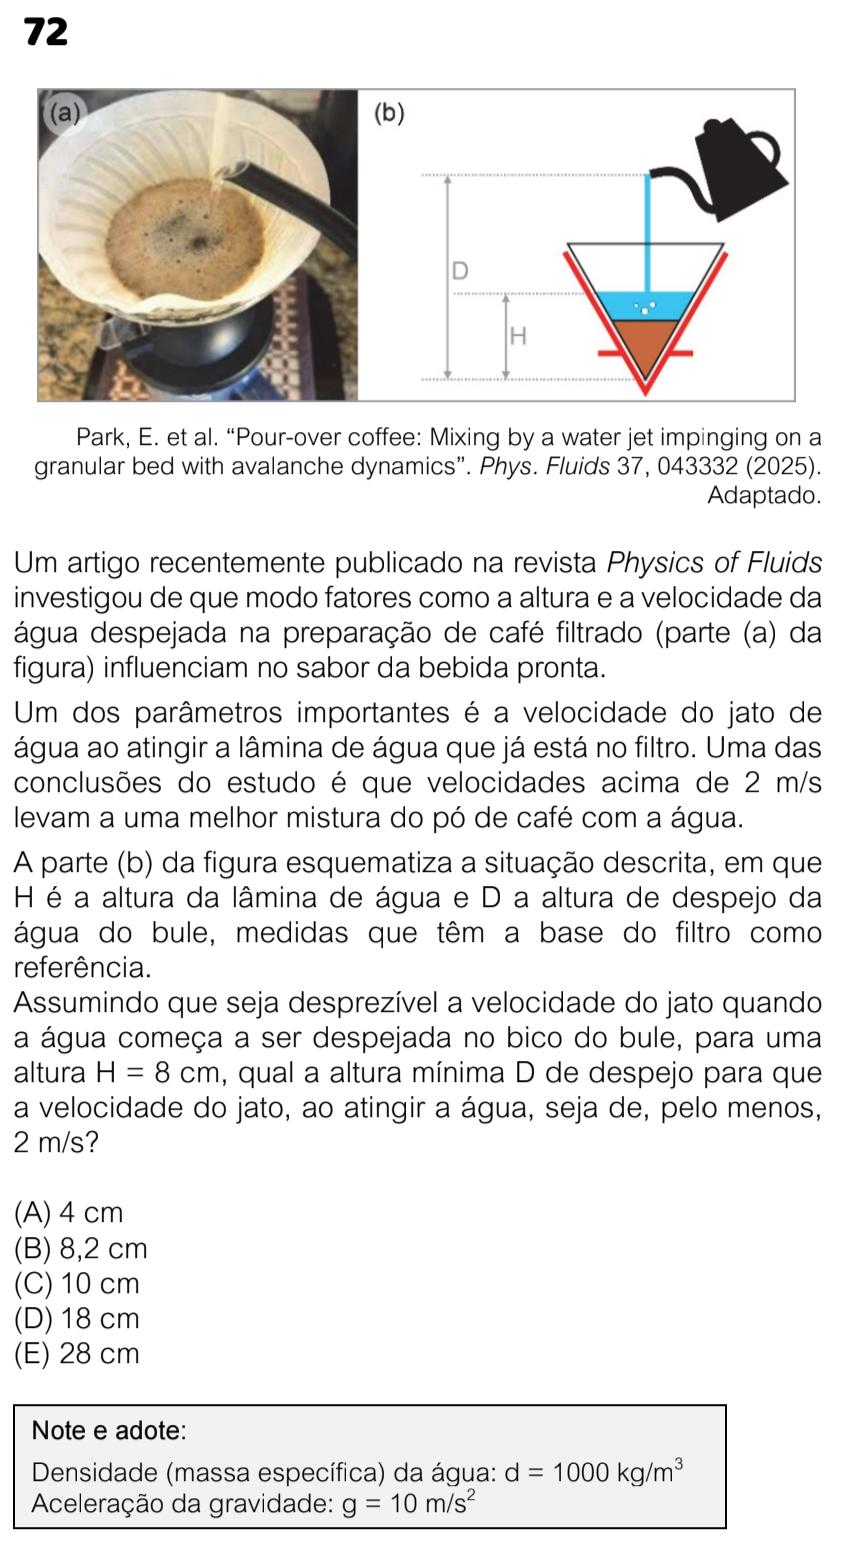
\includegraphics[width=0.75\textwidth]{images/2.png}
\caption{Esquema do preparo de café filtrado e alturas envolvidas.}
\end{figure}

\newpage

\begin{flushleft}

\textbf{\textcolor{blue}{\Large Quest\~ao 72}}\\

\vspace{0.3cm}

\textbf{Resolu\c{c}\~ao:}

\vspace{0.3cm}

O problema descreve a queda de um jato de água desde o bico do bule até a superfície da água no filtro. Como a velocidade inicial é desprezível, podemos modelar o movimento como uma \textbf{queda livre}, aplicando a conservação da energia mecânica.

\vspace{0.3cm}

A diferença de altura percorrida pela água é:
\[
\Delta h = D - H
\]

onde:
\begin{itemize}
\item \(D\): altura de despejo da água
\item \(H = 8 \, \text{cm}\): altura da lâmina de água
\end{itemize}

\vspace{0.3cm}

Pela conservação da energia mecânica:
\[
E_p = E_c
\]

\[
m g (D - H) = \frac{1}{2} m v^2
\]

Cancelando a massa \(m\):
\[
g (D - H) = \frac{1}{2} v^2
\]

\vspace{0.3cm}

Isolando a altura:
\[
D - H = \frac{v^2}{2g}
\]

Substituindo os valores fornecidos:
\[
v = 2 \, \text{m/s}, \quad g = 10 \, \text{m/s}^2
\]

\[
D - H = \frac{(2)^2}{2 \cdot 10} = \frac{4}{20} = 0{,}2 \, \text{m}
\]

Convertendo para centímetros:
\[
0{,}2 \, \text{m} = 20 \, \text{cm}
\]

\vspace{0.3cm}

Logo:
\[
D = H + 20
\]

\[
D = 8 + 20 = 28 \, \text{cm}
\]

\vspace{0.5cm}

\textcolor{red}{\textbf{Conclus\~ao:}}\\

A altura mínima de despejo para que a velocidade do jato ao atingir a água seja de pelo menos \(2 \, \text{m/s}\) é:

\[
\boxed{28 \, \text{cm}}
\]

\vspace{0.3cm}

Portanto, a alternativa correta é \textbf{(E)}.

\end{flushleft}

%%%%%%%% Bibliography 
% Os comandos para incluir as referências bibliográficas
%\printingbibliography

\end{document}
